 To see how good of a fit these parameters actually are we can look at the goodness of fit fo the asymetry in figure \ref{fig:asymVariation}, the matched orbit for stretch 1 of measurement 1 figure \ref{fig:orbitVariation} and the starting position (initial $\psi$) for that orbit in figure \ref{fig:initVariation}.  
 
 \begin{figure}[H]
 \begin{center}
 \includegraphics[width=0.7\textwidth]{figures/results/particleA/A_assymVariation.pdf}
 \end{center}
 \caption{We see how the difference between the theoretical $n_z$ and all the measured  $\widetilde{n_z}$ for all measurements of particle A for different asymmetries $\epsilon$. For each asymmetry we find the orbit and the initial $\psi$ with the smallest distance for each stretch.}
 \label{fig:asymVariation}
 \end{figure}
 
 \begin{figure}[H]
 \begin{center}
 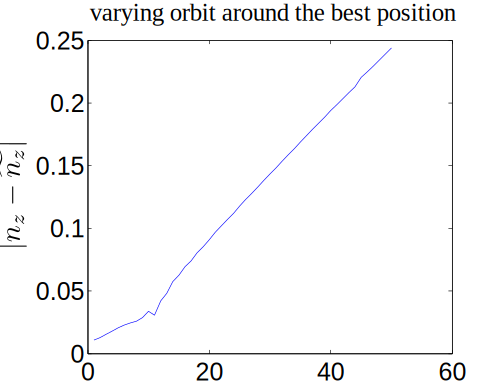
\includegraphics[width=0.7\textwidth]{figures/results/particleA/A_orbitVariation.pdf}
 \end{center}
 \caption{The difference between the theoretical $n_z$ and the measured $\widetilde{n_z}$ for the first stretch of the first measurement for particle A (seen in figure \ref{fig:particleA1})with the best asymmetry for different orbits. .}
 \label{fig:orbitVariation}
 \end{figure}
 
 
 \begin{figure}[H]
 \begin{center}
 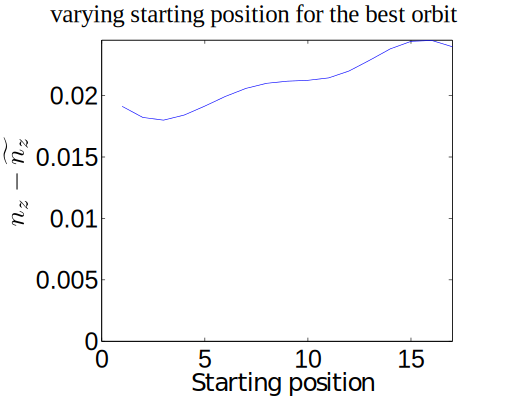
\includegraphics[width=0.7\textwidth]{figures/results/particleA/A_posVariation.pdf}
 \end{center}
 \caption{The difference between the theoretical $n_z$ and the measured $\widetilde{n_z}$ for the first stretch of the first measurement for particle A. The best orbit and best asymmetry are chosen, but different initial conditions are tested. }
 \label{fig:initVariation}
 \end{figure}
 
